% answers.tex —— 2009 年·普通高等学校招生考试·湖南卷·理科 · 参考答案与详细解析片段
% 由 tools/generate_projects.py 依来源总账自 2009/2009_数学真题_湖南理_试题.md + 2009/2009_数学真题_湖南理_解析正文.md + 2009/2009_数学真题_湖南理_答案要点.md 生成，勿手改（改源 MD 后重跑）


\begin{gktip}
固定候选 PDF 仅含题面，无答案、解析和评分标准，原页亦未标分值；以下为非官方编者独立推导，官方答案字段为空。分数、根号、上下标与三幅图均以 600 dpi 原页复核。原页第 4 题选项（A）（B）把 $\lambda_2$ 印成 $\lambda$、第 5 题「种数位」应为「种数为」、第 12 题「为原点的四边形」应为「为顶点的四边形」，均为排印问题；解析按更正后的语义理解，答案不受影响。第 18 题若取端点 $E=A_1$，虽仍有 $DE\perp AE$，但平面 $ADA_1$ 不与平面 $ACC_1A_1$ 垂直，题设结论不成立；按「$E$ 在 $A_1C_1$ 上」通常指内点的约定取内点，答案唯一。
\end{gktip}

\begin{answer}
\gksolhead{1}{}

\textbf{题目}：

若 $\log_2 a<0$，$\left(\dfrac12\right)^b>1$，则（　）

（A）$a>1$，$b>0$

（B）$a>1$，$b<0$

（C）$0<a<1$，$b>0$

（D）$0<a<1$，$b<0$

\Needspace{4\baselineskip}
\textbf{解析}

由 $\log_2a<0=\log_21$，对数函数 $\log_2x$ 在 $(0,+\infty)$ 上递增，故 $0<a<1$。

由 $\left(\dfrac12\right)^b>1=\left(\dfrac12\right)^0$，指数函数 $\left(\dfrac12\right)^x$ 在 $\mathbf R$ 上递减，故 $b<0$。选（D）。

\gkanswer{答案：D。}

\end{answer}
\begin{answer}
\gksolhead{2}{}

\textbf{题目}：

对于非零向量 $\boldsymbol a$，$\boldsymbol b$，“$\boldsymbol a+\boldsymbol b=\boldsymbol 0$”是“$\boldsymbol a\parallel\boldsymbol b$”的（　）

（A）充分不必要条件

（B）必要不充分条件

（C）充分必要条件

（D）既不充分也不必要条件

\Needspace{4\baselineskip}
\textbf{解析}

若 $\boldsymbol a+\boldsymbol b=\boldsymbol 0$，则 $\boldsymbol b=-\boldsymbol a$。因 $\boldsymbol a\neq\boldsymbol 0$，故 $\boldsymbol b$ 与 $\boldsymbol a$ 反向，$\boldsymbol a\parallel\boldsymbol b$，充分性成立。

反之，若 $\boldsymbol a\parallel\boldsymbol b$，只知两向量同向或反向。同向时（如 $\boldsymbol a=\boldsymbol b\neq\boldsymbol 0$）$\boldsymbol a+\boldsymbol b=2\boldsymbol a\neq\boldsymbol 0$，故必要性不成立。因此是充分不必要条件，选（A）。

\gkanswer{答案：A。}

\end{answer}
\begin{answer}
\gksolhead{3}{}

\textbf{题目}：

将函数 $y=\sin x$ 的图象向左平移 $\varphi$（$0\leqslant\varphi<2\pi$）个单位后，得到函数 $y=\sin\left(x-\dfrac\pi6\right)$ 的图象，则 $\varphi$ 等于（　）

（A）$\dfrac\pi6$

（B）$\dfrac{5\pi}6$

（C）$\dfrac{7\pi}6$

（D）$\dfrac{11\pi}6$

\Needspace{4\baselineskip}
\textbf{解析}

\Needspace{5\baselineskip}
$y=\sin x$ 的图象向左平移 $\varphi$ 个单位，所得图象对应

\nopagebreak[4]
\[y=\sin(x+\varphi).\]

\Needspace{5\baselineskip}
题设要求它与 $y=\sin\left(x-\dfrac\pi6\right)$ 是同一图象，故对一切 $x$，

\nopagebreak[4]
\[\sin(x+\varphi)=\sin\left(x-\frac\pi6\right),\]

\Needspace{5\baselineskip}
从而 $\varphi=-\dfrac\pi6+2k\pi$（$k\in\mathbf Z$）。由 $0\leqslant\varphi<2\pi$，取 $k=1$，得

\nopagebreak[4]
\[\varphi=2\pi-\frac\pi6=\frac{11\pi}6.\]

选（D）。检验：$\sin\left(x+\dfrac{11\pi}6\right)=\sin\left(x-\dfrac\pi6+2\pi\right)=\sin\left(x-\dfrac\pi6\right)$。

\gkanswer{答案：D。}

\end{answer}
\begin{answer}
\gksolhead{4}{}

\textbf{题目}：

如图，当参数 $\lambda=\lambda_1$，$\lambda_2$ 时，连续函数 $y=\dfrac{x}{1+\lambda x}$（$x\geqslant0$）的图象分别对应曲线 $C_1$ 和 $C_2$，则（　）

（A）$0<\lambda_1<\lambda$

（B）$0<\lambda<\lambda_1$

（C）$\lambda_1<\lambda_2<0$

（D）$\lambda_2<\lambda_1<0$
\nopagebreak[4]
\begin{center}% 2009 年湖南卷理科第 4 题：函数 y=x/(1+λx)（x≥0）的两条曲线 C1、C2。
% 来源 PDF：普通高考/2009/2009湖南理.pdf，SHA-256 0237bd2509e6645937e3473eabb63dba69098024fb6f451cb44ef8ac0e3165c1。
% 原页：第 1 页（A3 三栏）第 1 栏中部，书页码 527。
% 重绘依据：曲线按 λ1>λ2>0 绘制（λ2=0.45、λ1=1.2），上方为 C2；只画第一象限，
%   与原页一致保留坐标轴箭头、原点 O 及 C1、C2 两个标注。
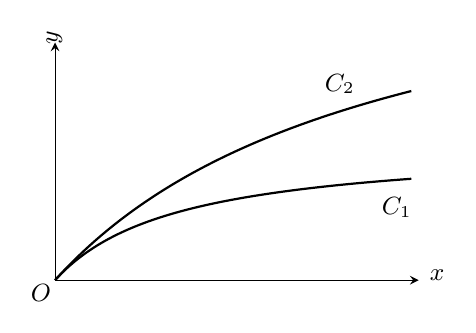
\begin{tikzpicture}[semithick, every node/.style={inner sep=1.2pt, font=\small}]
  \begin{axis}[
    width=6.2cm, height=4.6cm,
    axis lines=left,
    xmin=0, xmax=2.45, ymin=0, ymax=1.45,
    xtick=\empty, ytick=\empty,
    xlabel={$x$}, ylabel={$y$},
    xlabel style={at={(axis description cs:1.02,0.02)}, anchor=west},
    ylabel style={at={(axis description cs:0.03,1.02)}, anchor=south},
    axis line style={-stealth},
    clip=false,
  ]
    \addplot[domain=0:2.4, samples=120, thick] {x/(1+1.2*x)} node[pos=0.88, below right=4pt] {$C_1$};
    \addplot[domain=0:2.4, samples=120, thick] {x/(1+0.45*x)} node[pos=0.88, above left=2pt] {$C_2$};
    \node[below left] at (axis cs:0,0) {$O$};
  \end{axis}
\end{tikzpicture}
\end{center}
\nopagebreak[4]
\Needspace{4\baselineskip}
\textbf{解析}

\Needspace{5\baselineskip}
先看 $\lambda>0$ 的情形：

\nopagebreak[4]
\[y'=\frac{1\cdot(1+\lambda x)-x\cdot\lambda}{(1+\lambda x)^2}=\frac1{(1+\lambda x)^2}>0,\]

\nopagebreak[4]
\[y''=-\frac{2\lambda}{(1+\lambda x)^3}<0.\]

故曲线在 $x\geqslant0$ 上单调递增且上凸，并以 $y=\dfrac1\lambda$ 为水平渐近线，与原图的两条曲线形状一致。

\Needspace{5\baselineskip}
固定 $x>0$，函数 $\dfrac{x}{1+\lambda x}$ 关于 $\lambda$ 单调递减：$\lambda$ 越大，分母越大，函数值越小。图中 $C_2$ 在 $C_1$ 上方，故 $C_2$ 对应的参数较小，即 $\lambda_2<\lambda_1$。又二者均为正，得

\nopagebreak[4]
\[0<\lambda_2<\lambda_1.\]

原页（A）（B）把 $\lambda_2$ 印成 $\lambda$，按题设「$\lambda=\lambda_1,\lambda_2$」应读作 $\lambda_2$，故选（B）。

若 $\lambda<0$，则 $y''>0$，曲线下凸，且 $x\to-\dfrac1\lambda$ 时 $y\to+\infty$，与图中上凸的形状不符，故排除（C）（D）。

\gkanswer{答案：B。}

\end{answer}
\begin{answer}
\gksolhead{5}{}

\textbf{题目}：

从 $10$ 名大学毕业生中选 $3$ 个人担任村长助理，则甲、乙至少有 $1$ 人入选，而丙没有入选的不同选法的种数位（　）

（A）$85$

（B）$56$

（C）$49$

（D）$28$

\Needspace{4\baselineskip}
\textbf{解析}

丙没有入选，候选范围缩小为除丙外的 $9$ 人。

从 $9$ 人中任选 $3$ 人的总数为 $\mathrm C_9^3=84$。其中甲、乙都没有入选，即从其余 $7$ 人中选 $3$ 人，有 $\mathrm C_7^3=35$ 种。

\Needspace{5\baselineskip}
故甲、乙至少一人入选的选法为

\nopagebreak[4]
\[84-35=49.\]

选（C）。也可分类：恰有甲、乙之一入选 $2\mathrm C_7^2=42$ 种，甲、乙都入选 $\mathrm C_7^1=7$ 种，合计 $49$。

\gkanswer{答案：C。}

\end{answer}
\begin{answer}
\gksolhead{6}{}

\textbf{题目}：

已知 $D$ 是由不等式组 $\begin{cases}x-2y\geqslant0,\\ x+3y\geqslant0\end{cases}$ 所确定的平面区域，则圆 $x^2+y^2=4$ 在区域 $D$ 内的弧长为（　）

（A）$\dfrac\pi4$

（B）$\dfrac\pi2$

（C）$\dfrac{3\pi}4$

（D）$\dfrac{3\pi}2$

\Needspace{4\baselineskip}
\textbf{解析}

\Needspace{5\baselineskip}
区域 $D$ 由 $y\leqslant\dfrac x2$ 与 $y\geqslant-\dfrac x3$ 确定，是含正 $x$ 轴的一个角形区域。两条边界直线的斜率分别为 $\dfrac12$ 与 $-\dfrac13$，设夹角为 $\theta$，则

\nopagebreak[4]
\[\tan\theta=\left|\frac{\frac12-\left(-\frac13\right)}{1+\frac12\cdot\left(-\frac13\right)}\right|
=\frac{\frac56}{\frac56}=1,\]

故 $\theta=\dfrac\pi4$。

\Needspace{5\baselineskip}
圆 $x^2+y^2=4$ 的半径为 $2$，区域 $D$ 截圆所得弧的圆心角就是 $\dfrac\pi4$，弧长为

\nopagebreak[4]
\[l=r\theta=2\cdot\frac\pi4=\frac\pi2.\]

选（B）。检验：两射线与圆的交点分别为 $\left(\dfrac{4\sqrt5}5,\dfrac{2\sqrt5}5\right)$ 与 $\left(\dfrac{3\sqrt{10}}5,-\dfrac{\sqrt{10}}5\right)$，对应的圆心角为 $\arctan\dfrac12+\arctan\dfrac13$，由正切加法公式其和为 $\dfrac\pi4$。

\gkanswer{答案：B。}

\end{answer}
\begin{answer}
\gksolhead{7}{}

\textbf{题目}：

正方体 $ABCD-A_1B_1C_1D_1$ 的棱上到异面直线 $AB$，$CC_1$ 的距离相等的点的个数为（　）

（A）$2$

（B）$3$

（C）$4$

（D）$5$

\Needspace{4\baselineskip}
\textbf{解析}

\Needspace{5\baselineskip}
设正方体棱长为 $1$，建系

\nopagebreak[4]
\[A(0,0,0),\ B(1,0,0),\ C(1,1,0),\ D(0,1,0),\ C_1(1,1,1).\]

\Needspace{5\baselineskip}
直线 $AB$ 为 $y=z=0$；直线 $CC_1$ 为 $x=1$，$y=1$。点 $P(x,y,z)$ 到 $AB$ 的距离为

\nopagebreak[4]
\[d_1=\sqrt{y^2+z^2},\]

\Needspace{5\baselineskip}
到 $CC_1$ 的距离为

\nopagebreak[4]
\[d_2=\sqrt{(x-1)^2+(y-1)^2}.\]

\Needspace{5\baselineskip}
令 $d_1=d_2$，得

\nopagebreak[4]
\[y^2+z^2=(x-1)^2+(y-1)^2. \tag{$\ast$}\]

逐条棱检验：

\begin{itemize}
\item 棱 $AD$：$x=0$，$z=0$，$(\ast)$ 化为 $y^2=(y-1)^2$，得 $y=\dfrac12$，点为 $\left(0,\dfrac12,0\right)$。
\item 棱 $A_1D_1$：$x=0$，$z=1$，$(\ast)$ 化为 $y^2+1=(y-1)^2$，得 $y=\dfrac12$，点为 $\left(0,\dfrac12,1\right)$。
\item 棱 $BC$：$x=1$，$z=0$，$(\ast)$ 化为 $y^2=(y-1)^2$，得 $y=\dfrac12$，点为 $\left(1,\dfrac12,0\right)$。
\item 棱 $B_1C_1$：$x=1$，$z=1$，$(\ast)$ 化为 $y^2+1=(y-1)^2$，得 $y=\dfrac12$，点为 $\left(1,\dfrac12,1\right)$。
\item 棱 $DD_1$：$x=0$，$y=1$，$(\ast)$ 化为 $1+z^2=0$，无解。
\item 棱 $D_1C_1$：$y=1$，$z=1$，$(\ast)$ 化为 $1+1=(x-1)^2$，无棱内解。
\item 其余棱逐一代入均无解或解不在棱上。
\end{itemize}

注意 $D(0,1,0)$ 与 $B_1(1,0,1)$ 也满足 $(\ast)$：$D$ 到 $AB$、$CC_1$ 的距离都是 $1$，$B_1$ 到两线的距离也都是 $1$。它们分别是棱 $AD$、$DD_1$、$CD$ 与棱 $A_1B_1$、$B_1C_1$、$BB_1$ 的公共端点，在逐棱计数时已各计一次。

\Needspace{5\baselineskip}
合并重复端点，满足条件的点为

\nopagebreak[4]
\[D,\quad B_1,\quad \left(0,\frac12,1\right),\quad \left(1,\frac12,0\right),\]

共 $4$ 个。选（C）。

\gkanswer{答案：C。}

\end{answer}
\begin{answer}
\gksolhead{8}{}

\textbf{题目}：

\Needspace{5\baselineskip}
设函数 $y=f(x)$ 在 $(-\infty,+\infty)$ 内有定义．对于给定的正数 $K$，定义函数

\nopagebreak[4]
\[f_K(x)=\begin{cases}f(x),&f(x)\leqslant K,\\ K,&f(x)>K.\end{cases}\]

取函数 $f(x)=2-x-\mathrm e^{-x}$．若对任意的 $x\in(-\infty,+\infty)$，恒有 $f_K(x)=f(x)$，则（　）

（A）$K$ 的最大值为 $2$

（B）$K$ 的最小值为 $2$

（C）$K$ 的最大值为 $1$

（D）$K$ 的最小值为 $1$

\Needspace{4\baselineskip}
\textbf{解析}

\Needspace{5\baselineskip}
先求 $f(x)=2-x-\mathrm e^{-x}$ 的最大值：

\nopagebreak[4]
\[f'(x)=-1+\mathrm e^{-x}.\]

\Needspace{5\baselineskip}
令 $f'(x)=0$ 得 $\mathrm e^{-x}=1$，即 $x=0$。当 $x<0$ 时 $\mathrm e^{-x}>1$，$f'(x)>0$；当 $x>0$ 时 $f'(x)<0$。故 $f$ 在 $x=0$ 处取最大值

\nopagebreak[4]
\[f(0)=2-0-\mathrm e^0=1.\]

又 $x\to+\infty$ 时 $f(x)\to-\infty$，$x\to-\infty$ 时 $f(x)\to-\infty$，故 $f$ 的值域为 $(-\infty,1]$。

\Needspace{5\baselineskip}
按定义，$f_K(x)$ 在 $f(x)\leqslant K$ 时等于 $f(x)$，在 $f(x)>K$ 时被截为 $K$。要对一切 $x$ 都有 $f_K(x)=f(x)$，必须且只需

\nopagebreak[4]
\[K\geqslant\max f(x)=1.\]

因此 $K$ 的最小值为 $1$，无最大值（$K$ 可取任意不小于 $1$ 的数）。选（D）。

\gkanswer{答案：D。}

\end{answer}
\begin{answer}
\gksolhead{9}{}

\textbf{题目}：

某班共 $30$ 人，其中 $15$ 人喜爱篮球运动，$10$ 人喜爱乒乓球运动，$8$ 人对这两项运动都不喜爱，则喜爱篮球运动但不喜爱乒乓球运动的人数为$\underline{\qquad}$．

\Needspace{4\baselineskip}
\textbf{解析}

\Needspace{5\baselineskip}
设两项运动都喜爱的人数为 $t$。由容斥原理，至少喜爱一项的人数为 $15+10-t$，再加上两项都不喜爱的 $8$ 人，得

\nopagebreak[4]
\[15+10-t+8=30,\]

故 $t=3$。

喜爱篮球但不喜爱乒乓球的人数为 $15-3=12$。检验：只爱篮球 $12$ 人、只爱乒乓球 $7$ 人、两项都爱 $3$ 人、两项都不爱 $8$ 人，合计 $12+7+3+8=30$。

\gkanswer{答案：$12$。}

\end{answer}
\begin{answer}
\gksolhead{10}{}

\textbf{题目}：

在 $(1+x)^3+(1+x)^4+(1+\sqrt[3]{x})^3$ 的展开式中，$x$ 的系数为$\underline{\qquad}$．（用数字作答）

\Needspace{4\baselineskip}
\textbf{解析}

逐项取 $x$ 的一次项：

\begin{itemize}
\item $(1+x)^3$ 中 $x$ 的系数为 $\mathrm C_3^1=3$；
\item $(1+x)^4$ 中 $x$ 的系数为 $\mathrm C_4^1=4$；
\item $(1+\sqrt[3]x)^3$ 中，只有 $(\sqrt[3]x)^3=x$ 这一项，系数为 $\mathrm C_3^3=1$。
\end{itemize}

\Needspace{5\baselineskip}
故展开式中 $x$ 的系数为

\nopagebreak[4]
\[3+4+1=8.\]

\gkanswer{答案：$8$。}

\end{answer}
\begin{answer}
\gksolhead{11}{}

\textbf{题目}：

若 $x\in\left(0,\dfrac\pi2\right)$，则 $2\tan x+\tan\left(\dfrac\pi2-x\right)$ 的最小值为$\underline{\qquad}$．

\Needspace{4\baselineskip}
\textbf{解析}

\Needspace{5\baselineskip}
令 $t=\tan x$。由 $x\in\left(0,\dfrac\pi2\right)$ 得 $t>0$，且

\nopagebreak[4]
\[\tan\left(\frac\pi2-x\right)=\frac1{\tan x}=\frac1t.\]

\Needspace{5\baselineskip}
于是

\nopagebreak[4]
\[2\tan x+\tan\left(\frac\pi2-x\right)=2t+\frac1t.\]

\Needspace{5\baselineskip}
由基本不等式，

\nopagebreak[4]
\[2t+\frac1t\geqslant2\sqrt{2t\cdot\frac1t}=2\sqrt2,\]

当且仅当 $2t=\dfrac1t$，即 $t^2=\dfrac12$、$t=\dfrac{\sqrt2}2$ 时取等号。此时 $x=\arctan\dfrac{\sqrt2}2\in\left(0,\dfrac\pi2\right)$，故最小值 $2\sqrt2$ 可取到。

\gkanswer{答案：$2\sqrt2$。}

\end{answer}
\begin{answer}
\gksolhead{12}{}

\textbf{题目}：

已知以双曲线 $C$ 的两个焦点及虚轴的两个端点为原点的四边形中，有一个内角为 $60^\circ$，则双曲线 $C$ 的离心率为$\underline{\qquad}$．

\Needspace{4\baselineskip}
\textbf{解析}

双曲线设为 $\dfrac{x^2}{a^2}-\dfrac{y^2}{b^2}=1$，焦点 $(\pm c,0)$，虚轴端点 $(0,\pm b)$，其中 $c^2=a^2+b^2$。

\Needspace{5\baselineskip}
以这四点为顶点的四边形是菱形，对角线长分别为 $2c$ 与 $2b$。设焦点处内角为 $\theta$，则

\nopagebreak[4]
\[\tan\frac\theta2=\frac bc.\]

\Needspace{5\baselineskip}
因 $c>b$，$\dfrac bc<1$，故 $\theta<90^\circ$；而虚轴端点处内角为 $180^\circ-\theta>90^\circ$。因此题设的 $60^\circ$ 内角只能是焦点处的角，$\dfrac\theta2=30^\circ$，

\nopagebreak[4]
\[\frac bc=\tan30^\circ=\frac1{\sqrt3},\qquad c=\sqrt3 b.\]

\Needspace{5\baselineskip}
于是

\nopagebreak[4]
\[a^2=c^2-b^2=3b^2-b^2=2b^2,\]

\nopagebreak[4]
\[e=\frac ca=\frac{\sqrt3 b}{\sqrt2 b}=\frac{\sqrt6}2.\]

检验：此时 $\tan\dfrac\theta2=\dfrac1{\sqrt3}$，$\theta=60^\circ$，与题设一致。

\gkanswer{答案：$\dfrac{\sqrt6}{2}$。}

\end{answer}
\begin{answer}
\gksolhead{13}{}

\textbf{题目}：

一个总体分为 $A$，$B$ 两层，其个体数之比为 $4:1$，用分层抽样方法从总体中抽取一个容量为 $10$ 的样本．已知 $B$ 层中甲、乙都被抽到的概率为 $\dfrac1{28}$，则总体中的个体数为$\underline{\qquad}$．

\Needspace{4\baselineskip}
\textbf{解析}

\Needspace{5\baselineskip}
按个体数 $4:1$ 分层，样本容量 $10$，故 $B$ 层应抽

\nopagebreak[4]
\[10\times\frac1{4+1}=2\text{ \text{人}}.\]

\Needspace{5\baselineskip}
设 $B$ 层共有 $N$ 人，从中抽 $2$ 人。甲、乙都被抽到只有一种组合，故概率为

\nopagebreak[4]
\[\frac1{\mathrm C_N^2}=\frac1{28}.\]

于是 $\mathrm C_N^2=28$，即 $\dfrac{N(N-1)}2=28$，$N^2-N-56=0$，解得 $N=8$（负根舍去）。

总体人数为 $8\times(4+1)=40$。检验：$A$ 层 $32$ 人，抽 $8$ 人；$B$ 层 $8$ 人，抽 $2$ 人，合计 $10$ 人，比例 $8:2=4:1$。

\gkanswer{答案：$40$。}

\end{answer}
\begin{answer}
\gksolhead{14}{}

\textbf{题目}：

在半径为 $13$ 的球面上有 $A$，$B$，$C$ 三点，$AB=6$，$BC=8$，$CA=10$，则

（1）球心到平面 $ABC$ 的距离为$\underline{\qquad}$；

（2）过 $A$，$B$ 两点的大圆面与平面 $ABC$ 所成二面角（锐角）的正切值为$\underline{\qquad}$．

\Needspace{4\baselineskip}
\textbf{解析}

\Needspace{5\baselineskip}
（1）在 $\triangle ABC$ 中，$6^2+8^2=36+64=100=10^2$，即

\nopagebreak[4]
\[AB^2+BC^2=CA^2,\]

\Needspace{5\baselineskip}
故 $\triangle ABC$ 是以 $AC$ 为斜边的直角三角形，其外接圆圆心为 $AC$ 中点，半径

\nopagebreak[4]
\[r=\frac{AC}2=5.\]

\Needspace{5\baselineskip}
设球心为 $O$，$O$ 在平面 $ABC$ 上的射影为 $H$。球半径 $R=13$，$H$ 就是 $\triangle ABC$ 的外心，故 $HA=r=5$。于是球心到平面的距离

\nopagebreak[4]
\[OH=\sqrt{R^2-r^2}=\sqrt{13^2-5^2}=\sqrt{144}=12.\]

（2）设 $AC$ 中点为 $M$，则 $M=H$。在直角三角形中，$M$ 到 $AB$ 的距离等于 $\dfrac{BC}2=4$（中位线）。

\Needspace{5\baselineskip}
过 $A$，$B$ 的大圆面含球心 $O$ 与弦 $AB$。该平面与平面 $ABC$ 的交线为 $AB$。在垂直于 $AB$ 的截面内，$O$ 到平面 $ABC$ 的距离为 $OH=12$，$H$ 到 $AB$ 的距离为 $4$，二面角的平面角 $\alpha$ 满足

\nopagebreak[4]
\[\tan\alpha=\frac{OH}{4}=\frac{12}{4}=3.\]

故所求正切值为 $3$。

\gkanswer{答案：（1）$12$；（2）$3$。}

\end{answer}
\begin{answer}
\gksolhead{15}{}

\textbf{题目}：

将正 $\triangle ABC$ 分割成 $n^2$（$n\geqslant2$，$n\in\mathbf N^*$）个全等的小正三角形（图 1，图 2 分别给出了 $n=2$，$3$ 的情形），在每个三角形的顶点各放置一个数，使位于 $\triangle ABC$ 的三边及平行于某边的任一直线上的数（当数的个数不少于 $3$ 时）都分别依次成等差数列．若顶点 $A$，$B$，$C$ 处的三个数互不相同且和为 $1$，记所有顶点上的数之和为 $f(n)$，则有 $f(2)=2$，$f(3)=\underline{\qquad}$，$\cdots$，$f(n)=\underline{\qquad}$．
\nopagebreak[4]
\begin{center}% 2009 年湖南卷理科第 15 题：正三角形分割成 n^2 个小正三角形（n=2,3）。
% 来源 PDF：普通高考/2009/2009湖南理.pdf，SHA-256 0237bd2509e6645937e3473eabb63dba69098024fb6f451cb44ef8ac0e3165c1。
% 原页：第 1 页（A3 三栏）第 2 栏下部，书页码 527。
% 重绘依据：按原页两幅图重绘；左图 n=2 连接三边中点，右图 n=3 连接各边三等分点并作三组平行线。
\begin{tikzpicture}[semithick, every node/.style={inner sep=1.4pt, font=\small}]
  % 左图 n=2
  \coordinate (A) at (0,3.464);
  \coordinate (B) at (-2,0);
  \coordinate (C) at (2,0);
  \coordinate (MAB) at (-1,1.732);
  \coordinate (MBC) at (0,0);
  \coordinate (MCA) at (1,1.732);
  \draw (A) -- (B) -- (C) -- cycle;
  \draw (MAB) -- (MBC) -- (MCA) -- cycle;
  \node[above] at (A) {$A$};
  \node[below left] at (B) {$B$};
  \node[below right] at (C) {$C$};
  \node[below] at (0,-0.42) {图 1};

  % 右图 n=3
  \begin{scope}[xshift=1.0cm]
  \coordinate (A2) at (5,3.464);
  \coordinate (B2) at (3,0);
  \coordinate (C2) at (7,0);
  \coordinate (AB1) at (4.333,2.309);
  \coordinate (AB2) at (3.667,1.155);
  \coordinate (AC1) at (5.667,2.309);
  \coordinate (AC2) at (6.333,1.155);
  \coordinate (BC1) at (4.333,0);
  \coordinate (BC2) at (5.667,0);
  \draw (A2) -- (B2) -- (C2) -- cycle;
  % 平行于 BC 的两条
  \draw (AB1) -- (AC1);
  \draw (AB2) -- (AC2);
  % 平行于 AB 的两条
  \draw (AC1) -- (BC1);
  \draw (AC2) -- (BC2);
  % 平行于 AC 的两条
  \draw (AB1) -- (BC2);
  \draw (AB2) -- (BC1);
  \node[above] at (A2) {$A$};
  \node[below left] at (B2) {$B$};
  \node[below right] at (C2) {$C$};
  \node[below] at (5,-0.42) {图 2};
  \end{scope}
\end{tikzpicture}
\end{center}
\nopagebreak[4]
\Needspace{4\baselineskip}
\textbf{解析}

\Needspace{5\baselineskip}
第 $n$ 层三角形每边被分成 $n$ 段，格点总数为

\nopagebreak[4]
\[\frac{(n+1)(n+2)}2.\]

\Needspace{5\baselineskip}
给每个格点标重心坐标 $(i,j,k)$，其中 $i,j,k$ 为非负整数且 $i+j+k=n$，该点到 $BC$、$CA$、$AB$ 的距离比等于 $i:j:k$。设顶点 $A$，$B$，$C$ 处的数分别为 $a$，$b$，$c$。由三边及平行于某边的直线上各数成等差数列，格点 $(i,j,k)$ 处的数为

\nopagebreak[4]
\[x_{i,j,k}=\frac{ia+jb+kc}{n}.\]

（沿平行于 $BC$ 的直线，$i$ 固定，$x$ 随 $j,k$ 线性变化；沿三边亦同，故上式是满足全部等差条件的唯一填法。）

\Needspace{5\baselineskip}
于是

\nopagebreak[4]
\[f(n)=\sum_{i+j+k=n}\frac{ia+jb+kc}{n}
=\frac1n\left(a\sum i+b\sum j+c\sum k\right).\]

\Needspace{5\baselineskip}
由对称性三个和相等，且

\nopagebreak[4]
\[\sum i=\sum_{i=0}^n i(n-i+1)=(n+1)\frac{n(n+1)}2-\frac{n(n+1)(2n+1)}6
=\frac{n(n+1)(n+2)}6.\]

\Needspace{5\baselineskip}
又 $a+b+c=1$，故

\nopagebreak[4]
\[f(n)=\frac1n\cdot3\cdot\frac{n(n+1)(n+2)}6\cdot\frac13
=\frac{(n+1)(n+2)}6.\]

\Needspace{5\baselineskip}
令 $n=3$ 得

\nopagebreak[4]
\[f(3)=\frac{4\times5}6=\frac{10}3.\]

检验 $n=2$：$f(2)=\dfrac{3\times4}6=2$，与题设给出的 $f(2)=2$ 一致；取 $a=1$，$b=c=0$ 时六个顶点上的数为 $1,\dfrac12,0,\dfrac12,0,0$，和为 $2$，亦一致。

\gkanswer{答案：$\dfrac{10}{3}$；$\dfrac{(n+1)(n+2)}6$。}

\end{answer}
\begin{answer}
\gksolhead{16}{}

\textbf{题目}：

在 $\triangle ABC$ 中，已知 $2\overrightarrow{AB}\cdot\overrightarrow{AC}=\sqrt3\left|\overrightarrow{AB}\right|\cdot\left|\overrightarrow{AC}\right|=3\overrightarrow{BC}^2$，求角 $A$，$B$，$C$ 的大小．

\Needspace{4\baselineskip}
\textbf{解析}

记 $a=BC$，$b=CA$，$c=AB$。

\Needspace{5\baselineskip}
由 $2\overrightarrow{AB}\cdot\overrightarrow{AC}=\sqrt3|\overrightarrow{AB}|\cdot|\overrightarrow{AC}|$，即

\nopagebreak[4]
\[2bc\cos A=\sqrt3 bc.\]

\Needspace{5\baselineskip}
因 $b,c>0$，得

\nopagebreak[4]
\[\cos A=\frac{\sqrt3}2,\qquad A=30^\circ.\]

\Needspace{5\baselineskip}
又由 $\sqrt3|\overrightarrow{AB}|\cdot|\overrightarrow{AC}|=3\overrightarrow{BC}^2$ 得

\nopagebreak[4]
\[\sqrt3 bc=3a^2,\qquad a^2=\frac{bc}{\sqrt3}.\]

\Needspace{5\baselineskip}
由余弦定理，

\nopagebreak[4]
\[a^2=b^2+c^2-2bc\cos A=b^2+c^2-\sqrt3 bc.\]

\Needspace{5\baselineskip}
两式联立：

\nopagebreak[4]
\[b^2+c^2-\sqrt3 bc=\frac{bc}{\sqrt3},\qquad b^2+c^2=\frac4{\sqrt3}bc.\]

\Needspace{5\baselineskip}
令 $t=\dfrac bc>0$，两边除以 $c^2$：

\nopagebreak[4]
\[t^2+1=\frac4{\sqrt3}t,\qquad t^2-\frac4{\sqrt3}t+1=0.\]

\Needspace{5\baselineskip}
判别式 $\dfrac{16}3-4=\dfrac43$，故

\nopagebreak[4]
\[t=\frac{\frac4{\sqrt3}\pm\frac2{\sqrt3}}2=\sqrt3\ \text{\text{或}}\ \frac1{\sqrt3}.\]

若 $b=\sqrt3 c$，则 $a^2=\dfrac{\sqrt3 c\cdot c}{\sqrt3}=c^2$，$a=c$，故 $A=C=30^\circ$，$B=180^\circ-60^\circ=120^\circ$。

若 $b=\dfrac c{\sqrt3}$，则 $a^2=\dfrac{c^2/\sqrt3}{\sqrt3}=\dfrac{c^2}3$，结合 $b^2=\dfrac{c^2}3$ 得 $a=b$，故 $A=B=30^\circ$，$C=120^\circ$。

\Needspace{5\baselineskip}
两组均满足 $A=30^\circ$ 及题设向量等式，故

\nopagebreak[4]
\[(A,B,C)=(30^\circ,120^\circ,30^\circ)\ \text{\text{或}}\ (30^\circ,30^\circ,120^\circ).\]

\gkanswer{答案：$A=30^\circ$，$B=120^\circ$，$C=30^\circ$，或 $B=30^\circ$，$C=120^\circ$。}

\end{answer}
\begin{answer}
\gksolhead{17}{}

\textbf{题目}：

为拉动经济增长，某市决定新建一批重点工程，分别为基础设施工程、民生工程和产业建设工程三类．这三类工程所含项目的个数分别占总数的 $\dfrac12$，$\dfrac13$，$\dfrac16$．现在 $3$ 名工人独立地从中任选一个项目参与建设．

（1）求他们选择的项目所属类别互不相同的概率；

（2）记 $\xi$ 为 $3$ 人中选择的项目属于基础设施工程或产业建设工程的人数，求 $\xi$ 的分布列及数学期望．

\Needspace{4\baselineskip}
\textbf{解析}

\Needspace{5\baselineskip}
（1）三类项目被选中的概率分别为 $\dfrac12$，$\dfrac13$，$\dfrac16$。三人所选类别互不相同，即三类各有一人选中。先确定三人各自对应的类别，有 $3!$ 种；再乘各类被选中的概率：

\nopagebreak[4]
\[P=3!\cdot\frac12\cdot\frac13\cdot\frac16=6\cdot\frac1{36}=\frac16.\]

\Needspace{5\baselineskip}
（2）每人选择基础设施工程或产业建设工程的概率为

\nopagebreak[4]
\[p=\frac12+\frac16=\frac23,\]

\Needspace{5\baselineskip}
且各人独立选择，故 $\xi\sim B\left(3,\dfrac23\right)$。于是

\nopagebreak[4]
\[P(\xi=k)=\mathrm C_3^k\left(\frac23\right)^k\left(\frac13\right)^{3-k},\qquad k=0,1,2,3.\]

\Needspace{5\baselineskip}
逐项计算：

\nopagebreak[4]
\[P(\xi=0)=\left(\frac13\right)^3=\frac1{27},\qquad
P(\xi=1)=3\cdot\frac23\cdot\frac19=\frac6{27}=\frac29,\]

\nopagebreak[4]
\[P(\xi=2)=3\cdot\frac49\cdot\frac13=\frac{12}{27}=\frac49,\qquad
P(\xi=3)=\left(\frac23\right)^3=\frac8{27}.\]

分布列：

\begin{center}
\begin{tabular}{lllll}
\toprule
$\xi$ & $0$ & $1$ & $2$ & $3$ \\
\midrule
$P$ & $\dfrac1{27}$ & $\dfrac29$ & $\dfrac49$ & $\dfrac8{27}$ \\
\bottomrule
\end{tabular}
\end{center}

\Needspace{5\baselineskip}
数学期望

\nopagebreak[4]
\[E\xi=3\cdot\frac23=2.\]

也可用定义验证：$0\cdot\dfrac1{27}+1\cdot\dfrac6{27}+2\cdot\dfrac{12}{27}+3\cdot\dfrac8{27}=\dfrac{6+24+24}{27}=2$。

\gkanswer{答案：（1）$\dfrac16$；（2）分布列 $\dfrac1{27}$，$\dfrac29$，$\dfrac49$，$\dfrac8{27}$，$E\xi=2$。}

\end{answer}
\begin{answer}
\gksolhead{18}{}

\textbf{题目}：

如图，在正三棱柱 $ABC-A_1B_1C_1$ 中，$AB=\sqrt2 AA_1$．点 $D$ 是 $A_1B_1$ 的中点，点 $E$ 在 $A_1C_1$ 上，且 $DE\perp AE$．

（1）证明：平面 $ADE\perp$ 平面 $ACC_1A_1$；

（2）求直线 $AD$ 和平面 $ABC_1$ 所成角的正弦值．
\nopagebreak[4]
\begin{center}% 2009 年湖南卷理科第 18 题：正三棱柱 ABC-A1B1C1，D 为 A1B1 中点，E 在 A1C1 上且 DE⊥AE。
% 来源 PDF：普通高考/2009/2009湖南理.pdf，SHA-256 0237bd2509e6645937e3473eabb63dba69098024fb6f451cb44ef8ac0e3165c1。
% 原页：第 1 页（A3 三栏）第 3 栏中部，书页码 527。
% 重绘依据：按原页斜视方向重绘；正三棱柱底面边长 AB=4、侧棱 AA1=2√2（图上按示意比例）。
%   可见：A1A、AB、BB1、A1B1、A1C1、C1B1 为实线；被遮挡的 AC、CC1、CB 为虚线。
%   辅助线 A1D、A1E、AD、AE、DE 按原页画虚线；D 在 A1B1 上，E 在 A1C1 上（AE:EC≈1:3）。
%   投影取 (x,y,z) -> (x+0.13y, z+0.45y)。
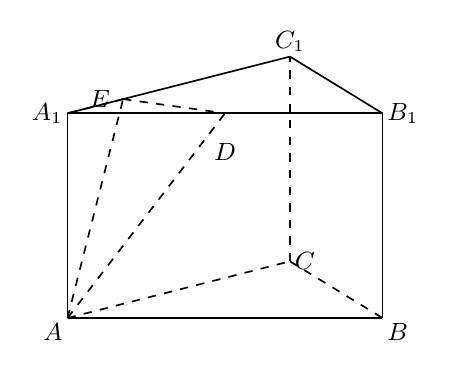
\begin{tikzpicture}[semithick, every node/.style={inner sep=1.5pt, font=\small}]
  \coordinate (A)  at (0.000,0.000);
  \coordinate (B)  at (4.000,0.000);
  \coordinate (C)  at (2.825,0.720);
  \coordinate (A1) at (0.000,2.600);
  \coordinate (B1) at (4.000,2.600);
  \coordinate (C1) at (2.825,3.320);
  \coordinate (D)  at (2.000,2.600);
  \coordinate (E)  at (0.706,2.780);

  % 可见棱
  \draw (A1) -- (A);
  \draw (A) -- (B);
  \draw (B) -- (B1);
  \draw (A1) -- (B1);
  \draw (A1) -- (C1);
  \draw (C1) -- (B1);

  % 被遮挡的棱
  \draw[dashed] (A) -- (C);
  \draw[dashed] (C) -- (C1);
  \draw[dashed] (C) -- (B);

  % 辅助线
  \draw[dashed] (A1) -- (D);
  \draw[dashed] (A1) -- (E);
  \draw[dashed] (A) -- (D);
  \draw[dashed] (A) -- (E);
  \draw[dashed] (E) -- (D);

  % 标注
  \node[left] at (A1) {$A_1$};
  \node[right] at (B1) {$B_1$};
  \node[above] at (C1) {$C_1$};
  \node[below left] at (A) {$A$};
  \node[below right] at (B) {$B$};
  \node[right] at (C) {$C$};
  \node[below=9pt] at (D) {$D$};
  \node[left=3pt] at (E) {$E$};
\end{tikzpicture}
\end{center}
\nopagebreak[4]
\Needspace{4\baselineskip}
\textbf{解析}

\Needspace{5\baselineskip}
（1）不妨取 $AB=2$，则由 $AB=\sqrt2 AA_1$ 得 $AA_1=\sqrt2$。以 $A$ 为原点，$AB$ 所在直线为 $x$ 轴，平面 $ABC$ 为 $xOy$ 平面建立空间直角坐标系。正三角形 $ABC$ 的高为 $\sqrt3$，故

\nopagebreak[4]
\[A(0,0,0),\ B(2,0,0),\ C(1,\sqrt3,0),\]
\nopagebreak[4]
\[A_1(0,0,\sqrt2),\ B_1(2,0,\sqrt2),\ C_1(1,\sqrt3,\sqrt2).\]

\Needspace{5\baselineskip}
$D$ 为 $A_1B_1$ 的中点，故 $D(1,0,\sqrt2)$。设

\nopagebreak[4]
\[E(t,\sqrt3t,\sqrt2)\qquad(0\leqslant t\leqslant1),\]

\Needspace{5\baselineskip}
则

\nopagebreak[4]
\[\overrightarrow{DE}=(t-1,\sqrt3t,0),\qquad \overrightarrow{AE}=(t,\sqrt3t,\sqrt2).\]

\Needspace{5\baselineskip}
由 $DE\perp AE$ 得

\nopagebreak[4]
\[(t-1)t+3t^2+0=0,\qquad 4t^2-t=0.\]

\Needspace{5\baselineskip}
解得 $t=0$ 或 $t=\dfrac14$。$t=0$ 时 $E=A_1$，此时 $DE\perp AE$ 也成立，但平面 $ADE$ 就是平面 $ADA_1$，其法向量 $(0,1,0)$ 与平面 $ACC_1A_1$ 的法向量 $(\sqrt3,-1,0)$ 不垂直，题设结论不成立；故题设的 $E$ 应取 $A_1C_1$ 的内点，$t=0$ 舍去。于是

\nopagebreak[4]
\[E\left(\frac14,\frac{\sqrt3}4,\sqrt2\right),\qquad
\overrightarrow{DE}=\left(-\frac34,\frac{\sqrt3}4,0\right).\]

\Needspace{5\baselineskip}
平面 $ACC_1A_1$ 由 $\overrightarrow{AC}=(1,\sqrt3,0)$ 与 $\overrightarrow{AA_1}=(0,0,\sqrt2)$ 张成，其法向量

\nopagebreak[4]
\[\boldsymbol n_1=\overrightarrow{AC}\times\overrightarrow{AA_1}=(\sqrt3,-1,0).\]

\Needspace{5\baselineskip}
而

\nopagebreak[4]
\[\overrightarrow{DE}=-\frac{\sqrt3}4(\sqrt3,-1,0)=-\frac{\sqrt3}4\boldsymbol n_1,\]

\Needspace{5\baselineskip}
故 $DE\perp$ 平面 $ACC_1A_1$。又 $DE\subset$ 平面 $ADE$，所以

\nopagebreak[4]
\[\text{\text{平面} }ADE\perp\text{\text{平面} }ACC_1A_1.\]

\Needspace{5\baselineskip}
（2）$\overrightarrow{AD}=(1,0,\sqrt2)$。平面 $ABC_1$ 由

\nopagebreak[4]
\[\overrightarrow{AB}=(2,0,0),\qquad \overrightarrow{AC_1}=(1,\sqrt3,\sqrt2)\]

\Needspace{5\baselineskip}
张成，法向量

\nopagebreak[4]
\[\boldsymbol n=\overrightarrow{AB}\times\overrightarrow{AC_1}
=(0\cdot\sqrt2-0\cdot\sqrt3,\ 0\cdot1-2\cdot\sqrt2,\ 2\cdot\sqrt3-0)
=(0,-2\sqrt2,2\sqrt3).\]

\Needspace{5\baselineskip}
取 $\boldsymbol n=(0,-\sqrt2,\sqrt3)$，则 $|\boldsymbol n|=\sqrt{2+3}=\sqrt5$，$|\overrightarrow{AD}|=\sqrt{1+2}=\sqrt3$。设直线 $AD$ 与平面 $ABC_1$ 所成角为 $\theta$，则

\nopagebreak[4]
\[\sin\theta=\frac{|\overrightarrow{AD}\cdot\boldsymbol n|}{|\overrightarrow{AD}|\cdot|\boldsymbol n|}
=\frac{|0+0+\sqrt2\cdot\sqrt3|}{\sqrt3\cdot\sqrt5}
=\frac{\sqrt6}{\sqrt{15}}=\frac{\sqrt{10}}5.\]

\gkanswer{答案：（1）证明见解析；（2）$\dfrac{\sqrt{10}}5$。}

\end{answer}
\begin{answer}
\gksolhead{19}{}

\textbf{题目}：

某地建一座桥，两端的桥墩已建好，这两墩相距 $m$ 米，余下工程只需要建两端桥墩之间的桥面和桥墩．经测算，一个桥墩的工程费用为 $256$ 万元，距离为 $x$ 米的相邻两墩之间的桥面工程费用为 $(2+\sqrt x)x$ 万元．假设桥墩等距离分布，所有桥墩都视为点，且不考虑其他因素，记余下工程的费用为 $y$ 万元．

（1）试写出 $y$ 关于 $x$ 的函数关系式；

（2）当 $m=640$ 米时，需新建多少个桥墩才能使 $y$ 最小？

\Needspace{4\baselineskip}
\textbf{解析}

\Needspace{5\baselineskip}
（1）设新建 $n$ 个桥墩。两端桥墩已建好，加上新建的 $n$ 个，桥面共分成 $n+1$ 段，故

\nopagebreak[4]
\[x=\frac m{n+1},\qquad n+1=\frac mx,\qquad n=\frac mx-1.\]

\Needspace{5\baselineskip}
桥面工程费用为

\nopagebreak[4]
\[(n+1)(2+\sqrt x)x=\frac mx(2+\sqrt x)x=2m+m\sqrt x.\]

\Needspace{5\baselineskip}
桥墩工程费用为 $256n=256\left(\dfrac mx-1\right)$。故

\nopagebreak[4]
\[y=2m+m\sqrt x+256\left(\frac mx-1\right)
=m\sqrt x+\frac{256m}{x}+2m-256\qquad(x>0).\]

\Needspace{5\baselineskip}
（2）当 $m=640$ 时，

\nopagebreak[4]
\[y=640\sqrt x+\frac{163840}{x}+1024.\]

\Needspace{5\baselineskip}
求导：

\nopagebreak[4]
\[y'=640\cdot\frac1{2\sqrt x}-\frac{163840}{x^2}
=\frac{320}{\sqrt x}-\frac{163840}{x^2}.\]

\Needspace{5\baselineskip}
令 $y'=0$：

\nopagebreak[4]
\[\frac{320}{\sqrt x}=\frac{163840}{x^2},\qquad x^{3/2}=\frac{163840}{320}=512=8^3,\]

故 $x=64$。

当 $0<x<64$ 时，$x^{3/2}<512$，$y'<0$；当 $x>64$ 时，$y'>0$。故 $x=64$ 是极小值点，也是最小值点。

\Needspace{5\baselineskip}
此时新建桥墩数

\nopagebreak[4]
\[n=\frac{640}{64}-1=10-1=9.\]

检验：$x=64$ 时 $y=640\times8+\dfrac{163840}{64}+1024=5120+2560+1024=8704$ 万元。相邻整数情形中，$n=8$ 时 $x=\dfrac{640}9\approx71.11$，$y\approx8725$ 万元；$n=10$ 时 $x=\dfrac{640}{11}\approx58.18$，$y\approx8722$ 万元，均大于 $8704$，故 $n=9$ 确为最小值点。

\gkanswer{答案：（1）$y=m\sqrt x+\dfrac{256m}{x}+2m-256$（$x>0$）；（2）$9$ 个。}

\end{answer}
\begin{answer}
\gksolhead{20}{}

\textbf{题目}：

在平面直角坐标系 $xOy$ 中，点 $P$ 到点 $F(3,0)$ 的距离的 $4$ 倍与它到直线 $x=2$ 的距离的 $3$ 倍之和记为 $d$．当点 $P$ 运动时，$d$ 恒等于点 $P$ 的横坐标与 $18$ 之和．

（1）求点 $P$ 的轨迹 $C$；

（2）设过点 $F$ 的直线 $l$ 与轨迹 $C$ 相交于 $M$，$N$ 两点，求线段 $MN$ 长度的最大值．

\Needspace{4\baselineskip}
\textbf{解析}

\Needspace{5\baselineskip}
（1）设 $P(x,y)$，由题意

\nopagebreak[4]
\[4\sqrt{(x-3)^2+y^2}+3|x-2|=x+18. \tag{1}\]

\Needspace{5\baselineskip}
当 $x\geqslant2$ 时，$|x-2|=x-2$，代入得

\nopagebreak[4]
\[4\sqrt{(x-3)^2+y^2}=x+18-3(x-2)=24-2x,\]

\Needspace{5\baselineskip}
即

\nopagebreak[4]
\[2\sqrt{(x-3)^2+y^2}=12-x. \tag{2}\]

\Needspace{5\baselineskip}
（2）式要求 $12-x\geqslant0$，即 $x\leqslant12$。两边平方：

\nopagebreak[4]
\[4\left[(x-3)^2+y^2\right]=(12-x)^2,\]

\nopagebreak[4]
\[4(x^2-6x+9+y^2)=144-24x+x^2,\]

\nopagebreak[4]
\[4x^2-24x+36+4y^2=144-24x+x^2,\]

\nopagebreak[4]
\[3x^2+4y^2=108,\]

\Needspace{5\baselineskip}
即

\nopagebreak[4]
\[\frac{x^2}{36}+\frac{y^2}{27}=1\qquad(x\geqslant2). \tag{3}\]

\Needspace{5\baselineskip}
当 $x<2$ 时，$|x-2|=2-x$，代入得

\nopagebreak[4]
\[4\sqrt{(x-3)^2+y^2}=x+18-3(2-x)=4x+12,\]

\Needspace{5\baselineskip}
即

\nopagebreak[4]
\[\sqrt{(x-3)^2+y^2}=x+3. \tag{4}\]

\Needspace{5\baselineskip}
两边平方：

\nopagebreak[4]
\[(x-3)^2+y^2=(x+3)^2,\]

\nopagebreak[4]
\[x^2-6x+9+y^2=x^2+6x+9,\]

\nopagebreak[4]
\[y^2=12x. \tag{5}\]

（5）要求 $x\geqslant0$，结合 $x<2$ 得 $0\leqslant x<2$。

\Needspace{5\baselineskip}
故轨迹 $C$ 为

\nopagebreak[4]
\[\frac{x^2}{36}+\frac{y^2}{27}=1\ (2\leqslant x\leqslant6),\qquad
y^2=12x\ (0\leqslant x<2).\]

两段在 $x=2$ 处相接：椭圆上 $y^2=27\left(1-\dfrac4{36}\right)=24$，抛物线上 $y^2=24$，公共点为 $A(2,\pm2\sqrt6)$。

（2）设直线 $l$ 的斜率为 $k$，则 $l:y=k(x-3)$。

\Needspace{5\baselineskip}
先看直线与椭圆弧的两个交点。代入（3）：

\nopagebreak[4]
\[\frac{x^2}{36}+\frac{k^2(x-3)^2}{27}=1.\]

\Needspace{5\baselineskip}
两边乘 $108$：

\nopagebreak[4]
\[3x^2+4k^2(x-3)^2=108,\]

\nopagebreak[4]
\[(3+4k^2)x^2-24k^2x+36k^2-108=0. \tag{6}\]

\Needspace{5\baselineskip}
设两根为 $x_1,x_2$，则

\nopagebreak[4]
\[x_1+x_2=\frac{24k^2}{3+4k^2},\qquad
x_1x_2=\frac{36k^2-108}{3+4k^2}.\]

\Needspace{5\baselineskip}
弦长

\nopagebreak[4]
\[|MN|=\sqrt{1+k^2}\,|x_1-x_2|.\]

\Needspace{5\baselineskip}
判别式

\nopagebreak[4]
\[\Delta=(24k^2)^2-4(3+4k^2)(36k^2-108)=1296(1+k^2),\]

\Needspace{5\baselineskip}
故

\nopagebreak[4]
\[|x_1-x_2|=\frac{\sqrt\Delta}{3+4k^2}=\frac{36\sqrt{1+k^2}}{3+4k^2},\]

\nopagebreak[4]
\[|MN|=\frac{36(1+k^2)}{3+4k^2}=9+\frac9{3+4k^2}. \tag{7}\]

\Needspace{5\baselineskip}
（7）在椭圆弧的两个交点都满足 $x\geqslant2$ 时成立。由（6）的较大根随 $|k|$ 减小而增大、较小根随 $|k|$ 增大而增大，临界情形是较小根恰为 $x=2$。令 $x=2$ 代入（6）：

\nopagebreak[4]
\[4(3+4k^2)-48k^2+36k^2-108=0,\]

\nopagebreak[4]
\[12+16k^2-12k^2-108=0,\qquad 4k^2=96,\qquad k^2=24.\]

\Needspace{5\baselineskip}
故当 $k^2\geqslant24$ 时，两交点都在椭圆弧上，且由（7）知 $|MN|$ 随 $k^2$ 增大而减小，最大值在 $k^2=24$ 处取得：

\nopagebreak[4]
\[|MN|_{\max}^{\text{(ellipse)}}=9+\frac9{3+4\times24}
=9+\frac9{99}=9+\frac1{11}=\frac{100}{11}. \tag{8}\]

\Needspace{5\baselineskip}
当 $k^2<24$ 时，直线与椭圆弧只有一个交点（另一个交点的 $x<2$，不在轨迹上），另一个交点在抛物线弧上。此时直接求两交点距离：抛物线交点满足 $k^2(x-3)^2=12x$，即

\nopagebreak[4]
\[k^2x^2-(6k^2+12)x+9k^2=0. \tag{9}\]

对 $k=0$，直线 $y=0$ 与轨迹交于椭圆右顶点 $(6,0)$ 与抛物线顶点 $(0,0)$，$|MN|=6<\dfrac{100}{11}$。

对 $0<k^2<24$，令 $u=\sqrt{1+k^2}$，则 $1<u<5$，且 $k^2=u^2-1$。

\Needspace{5\baselineskip}
抛物线交点（取 $[0,2)$ 内的根）为

\nopagebreak[4]
\[x_p=\frac{3(u-1)}{u+1};\]

\Needspace{5\baselineskip}
椭圆弧上对应交点为

\nopagebreak[4]
\[x_e=\frac{6(2u^2+3u-2)}{4u^2-1}.\]

\Needspace{5\baselineskip}
两交点都在直线 $y=k(x-3)$ 上，故

\nopagebreak[4]
\[|MN|=u\,(x_e-x_p)
=\frac{3u(14u^2+3u-5)}{(4u^2-1)(u+1)}. \tag{10}\]

\Needspace{5\baselineskip}
要证 $|MN|\leqslant\dfrac{100}{11}$，因各因式为正，等价于

\nopagebreak[4]
\[33u(14u^2+3u-5)\leqslant100(4u^2-1)(u+1).\]

\Needspace{5\baselineskip}
移项并因式分解：

\nopagebreak[4]
\[100(4u^2-1)(u+1)-33u(14u^2+3u-5)
=(5-u)(62u^2+9u-20).\]

当 $1\leqslant u\leqslant5$ 时，$5-u\geqslant0$，且 $62u^2+9u-20\geqslant62+9-20=51>0$，故不等式成立，等号仅在 $u=5$（即 $k^2=24$）时取得。因此混合分支的 $|MN|$ 也以 $\dfrac{100}{11}$ 为上界；当 $k^2\to24^-$ 时，抛物线根趋于 $2$，距离连续趋于（8）的值。故全局最大值即（8）。

\Needspace{5\baselineskip}
等号在直线 $AF$ 处取得。以 $A(2,-2\sqrt6)$ 为例，直线 $AF$ 的斜率

\nopagebreak[4]
\[k=\frac{0-(-2\sqrt6)}{3-2}=2\sqrt6,\qquad k^2=24.\]

\Needspace{5\baselineskip}
将其代入（6）：

\nopagebreak[4]
\[99x^2-576x+756=0,\]

\Needspace{5\baselineskip}
即 $11x^2-64x+84=0$，两根为 $x=2$ 与 $x=\dfrac{42}{11}$。另一交点

\nopagebreak[4]
\[N\left(\frac{42}{11},\ 2\sqrt6\left(\frac{42}{11}-3\right)\right)
=\left(\frac{42}{11},\ \frac{18\sqrt6}{11}\right).\]

\Needspace{5\baselineskip}
于是

\nopagebreak[4]
\[|AN|=\sqrt{\left(\frac{42}{11}-2\right)^2+\left(\frac{18\sqrt6}{11}+2\sqrt6\right)^2}
=\sqrt{\left(\frac{20}{11}\right)^2+\left(\frac{40\sqrt6}{11}\right)^2}.\]

\nopagebreak[4]
\[|AN|=\frac{\sqrt{400+9600}}{11}=\frac{100}{11}.\]

\gkanswer{答案：（1）$\dfrac{x^2}{36}+\dfrac{y^2}{27}=1$（$x\geqslant2$），或 $y^2=12x$（$0\leqslant x<2$）；（2）$\dfrac{100}{11}$。}

\end{answer}
\begin{answer}
\gksolhead{21}{}

\textbf{题目}：

对于数列 $\{u_n\}$，若存在常数 $M>0$，对任意的 $n\in\mathbf N^*$，恒有 $|u_{n+1}-u_n|+|u_n-u_{n-1}|+\cdots+|u_2-u_1|\leqslant M$，则称数列 $\{u_n\}$ 为 $B-$数列．

（1）首项为 $1$，公比为 $q$（$|q|<1$）的等比数列是否为 $B-$数列？请说明理由；

（2）设 $S_n$ 是数列 $\{x_n\}$ 的前 $n$ 项和，给出下列两组论断：

$A$ 组：① 数列 $\{x_n\}$ 是 $B-$数列　② 数列 $\{x_n\}$ 不是 $B-$数列

$B$ 组：③ 数列 $\{S_n\}$ 是 $B-$数列　④ 数列 $\{S_n\}$ 不是 $B-$数列

请以其中一组中的一个论断为条件，另一组中的一个论断为结论组成一个命题．判断所给命题的真假，并证明你的结论；

（3）若数列 $\{a_n\}$，$\{b_n\}$ 都是 $B-$数列，证明：数列 $\{a_nb_n\}$ 也是 $B-$数列．

\Needspace{4\baselineskip}
\textbf{解析}

\Needspace{5\baselineskip}
（1）设 $u_n=q^{n-1}$，$|q|<1$。则

\nopagebreak[4]
\[|u_{k+1}-u_k|=|q^k-q^{k-1}|=|q|^{k-1}|q-1|.\]

\Needspace{5\baselineskip}
故对任意 $n\in\mathbf N^*$，

\nopagebreak[4]
\[\sum_{k=1}^n|u_{k+1}-u_k|
=|q-1|\sum_{k=1}^n|q|^{k-1}
=|1-q|\cdot\frac{1-|q|^n}{1-|q|}
<\frac{|1-q|}{1-|q|}.\]

右端是与 $n$ 无关的正常数，取 $M=\dfrac{|1-q|}{1-|q|}$（或任意更大的数），即满足 $B-$数列定义。故首项为 $1$、公比为 $q$（$|q|<1$）的等比数列是 $B-$数列。

（2）②$\Rightarrow$④ 为真命题。

\Needspace{5\baselineskip}
证明 ③$\Rightarrow$①：设 $\{S_n\}$ 是 $B-$数列，则存在 $M>0$，使对一切 $n$，

\nopagebreak[4]
\[\sum_{k=1}^n|S_{k+1}-S_k|\leqslant M.\]

\Needspace{5\baselineskip}
而 $S_{k+1}-S_k=x_{k+1}$，故 $\sum\limits_{k=1}^n|x_{k+1}|\leqslant M$，即 $\sum|x_n|$ 的部分和有界。又

\nopagebreak[4]
\[|x_{n+1}-x_n|\leqslant|x_{n+1}|+|x_n|,\]

\Needspace{5\baselineskip}
求和得

\nopagebreak[4]
\[\sum_{k=1}^n|x_{k+1}-x_k|
\leqslant\sum_{k=1}^n|x_{k+1}|+\sum_{k=1}^n|x_k|
\leqslant2M.\]

故 $\{x_n\}$ 是 $B-$数列。即 ③$\Rightarrow$①，其逆否命题为 ②$\Rightarrow$④，故 ②$\Rightarrow$④ 真。

其余三条为假，逐一举反例：

\begin{itemize}
\item ①$\Rightarrow$③：取 $x_n=1$。则 $|x_{n+1}-x_n|=0$，$\{x_n\}$ 是 $B-$数列；但 $S_n=n$，$|S_{n+1}-S_n|=1$，部分和 $n$ 无界，$\{S_n\}$ 不是 $B-$数列。
\item ①$\Rightarrow$④：取 $x_n=2^{1-n}$。则 $\sum|x_{n+1}-x_n|=\sum2^{-n}<1$，$\{x_n\}$ 是 $B-$数列；而 $S_n=2-2^{1-n}$，$\sum|S_{n+1}-S_n|=\sum2^{-n}<1$，$\{S_n\}$ 也是 $B-$数列，故结论④不成立。
\item ②$\Rightarrow$③：取 $x_n=(-1)^n$。则 $|x_{n+1}-x_n|=2$，$\{x_n\}$ 不是 $B-$数列；而 $S_n$ 在 $-1$ 与 $0$ 之间交替，$|S_{n+1}-S_n|=1$，$\{S_n\}$ 也不是 $B-$数列，故结论③不成立。
\end{itemize}

综上，四条命题中只有 ②$\Rightarrow$④（等价地 ③$\Rightarrow$①）为真。

\Needspace{5\baselineskip}
（3）设 $\{a_n\}$ 是 $B-$数列，常数为 $M_a$。由

\nopagebreak[4]
\[|a_n|\leqslant|a_1|+|a_n-a_1|
\leqslant|a_1|+\sum_{k=1}^{n-1}|a_{k+1}-a_k|
\leqslant|a_1|+M_a,\]

知 $\{a_n\}$ 有界，记 $A=|a_1|+M_a$。同理 $\{b_n\}$ 有界，记 $B=|b_1|+M_b$。

\Needspace{5\baselineskip}
对任意 $n$，

\nopagebreak[4]
\[|a_{n+1}b_{n+1}-a_nb_n|
=|a_{n+1}(b_{n+1}-b_n)+b_n(a_{n+1}-a_n)|\]

\nopagebreak[4]
\[\leqslant A|b_{n+1}-b_n|+B|a_{n+1}-a_n|.\]

\Needspace{5\baselineskip}
求和：

\nopagebreak[4]
\[\sum_{k=1}^n|a_{k+1}b_{k+1}-a_kb_k|
\leqslant A\sum_{k=1}^n|b_{k+1}-b_k|+B\sum_{k=1}^n|a_{k+1}-a_k|
\leqslant AM_b+BM_a.\]

取 $M'=AM_b+BM_a>0$，则对一切 $n$ 部分和不超过 $M'$，故 $\{a_nb_n\}$ 也是 $B-$数列。

\gkanswer{答案：（1）是；（2）②$\Rightarrow$④ 为真命题；（3）证明见解析。}

\end{answer}